\documentclass[11pt,a4paper]{article}

\usepackage[margin=1in]{geometry}
\usepackage{graphicx}
\usepackage{booktabs}
\usepackage{array}
\usepackage{longtable}
\usepackage{caption}
\usepackage{subcaption}
\usepackage{xcolor}
\usepackage{listings}
\usepackage{amsmath}
\usepackage{enumitem}
\usepackage{fancyhdr}
\usepackage{titlesec}
\usepackage[hidelinks]{hyperref}

\definecolor{codebg}{RGB}{245,245,245}
\definecolor{codekw}{RGB}{0,80,150}
\definecolor{codecomment}{RGB}{110,110,110}
\definecolor{codestring}{RGB}{140,20,20}

\lstset{
  backgroundcolor=\color{codebg},
  basicstyle=\ttfamily\small,
  keywordstyle=\color{codekw}\bfseries,
  commentstyle=\color{codecomment}\itshape,
  stringstyle=\color{codestring},
  showstringspaces=false,
  breaklines=true,
  frame=single,
  rulecolor=\color{gray!40},
  numbers=left,
  numberstyle=\tiny\color{gray},
  xleftmargin=1.8em,
  language=Python
}

\titleformat{\section}{\normalfont\Large\bfseries}{\thesection}{1em}{}
\titleformat{\subsection}{\normalfont\large\bfseries}{\thesubsection}{1em}{}

\pagestyle{fancy}
\fancyhf{}
\fancyhead[L]{ICS1512 -- Machine Learning Algorithms Laboratory}
\fancyhead[R]{Experiment 5}
\fancyfoot[C]{\thepage}
\renewcommand{\headrulewidth}{0.4pt}

\title{}
\date{}

\begin{document}

% ---------------- Title Page ----------------
\begin{titlepage}
\centering
\vspace*{1cm}
{\Large\bfseries Sri Sivasubramaniya Nadar College of Engineering, Chennai\par}
\vspace{0.2cm}
{\normalsize (An Autonomous Institution Affiliated to Anna University)\par}
\vspace{1.2cm}

{\Large\bfseries Machine Learning Algorithms Laboratory\par}
\vspace{0.3cm}
{\large ICS1512\par}
\vspace{1.5cm}

\begin{tabular}{|p{5.5cm}|p{7cm}|}
\hline
Degree \& Branch & M.Tech (Integrated) Computer Science \& Engineering \\
\hline
Semester & V \\
\hline
Academic Year & 2026--2027 (Odd) \\
\hline
Batch & 2024--2029 \\
\hline
\end{tabular}

\vspace{1.8cm}
{\Large\bfseries Experiment 5\par}
\vspace{0.3cm}
{\large Decision Tree and Random Forest: A Comparative Classification Study\footnote{\textbf{GitHub Repository: }\url{https://github.com/VijayaraaghavanKS/ML}}\par}
\vspace{2.5cm}

\begin{tabular}{ll}
Submitted by: & \textbf{Vijayaraaghavan K S} \\[4pt]
Register Number: & \textbf{3122247001066} \\[4pt]
Year: & III Year \\[4pt]
Programme: & M.Tech Integrated, CSE \\[4pt]
Faculty: & Dr. Poreddy Ajay Kumar Reddy \\[4pt]
\end{tabular}

\vfill
\end{titlepage}

\tableofcontents
\newpage

% ==========================================================
\section{Aim and Objective}
To implement a Decision Tree classifier and extend it into a Random Forest ensemble on the Wisconsin Diagnostic Breast Cancer dataset, tune both models with 5-fold cross-validated GridSearchCV, and study how tree depth and ensemble size trade off overfitting against generalization.

% ==========================================================
\section{Problem Statement}
The input is a 30-dimensional vector of numeric measurements describing the nuclei present in a digitized image of a breast mass (radius, texture, perimeter, area, smoothness, and related shape descriptors, each summarized as a mean, standard error, and ``worst'' value); the output is a binary diagnosis, malignant or benign. Where Experiment 4 asked whether a linear model or a kernel-based margin classifier makes better use of a fixed feature set, this experiment asks a related but different question: does building an ensemble of decorrelated trees actually buy anything over a single, carefully tuned tree once both are given the same 5-fold cross-validation budget to select their hyperparameters, or does a single tree already capture the decision boundary well enough on a dataset this size?

% ==========================================================
\section{Theory}

\subsection{Decision Tree}
A Decision Tree recursively partitions the feature space by choosing, at each node, the single feature and threshold that most reduces class impurity, measured either by the Gini index $G = 1-\sum_c p_c^2$ or by entropy $H = -\sum_c p_c\log_2 p_c$. Left unconstrained, the tree keeps splitting until every leaf is pure (or contains too few samples to split further), which lets it memorize the training set rather than learn a boundary that generalizes -- the classic high-variance failure mode of tree models.

\subsection{Random Forest}
A Random Forest trains many decision trees, each on an independent bootstrap resample of the training data, and additionally restricts every split to a random subset of the available features rather than letting each tree search all of them. Averaging predictions across trees that are individually noisy but only weakly correlated with each other (because both the data and the candidate features differ from tree to tree) reduces the variance of the ensemble well below that of any single constituent tree, without much cost to bias.

% ==========================================================
\section{Machine Learning Algorithm}

\subsection{Decision Tree}
\textbf{Working principle:} starting from the root, greedily pick the (feature, threshold) split that maximizes impurity reduction, recurse on each child, and stop once a stopping criterion (max depth, minimum samples per split/leaf, or a pure node) is reached.
\textbf{Mathematical formulation:} the split that maximizes information gain $IG = H(\text{parent}) - \sum_{k} \frac{n_k}{n} H(\text{child}_k)$ (entropy criterion) or the equivalent Gini-impurity reduction is chosen at every node; prediction at a leaf is the majority class of the training samples that fell into it.
\textbf{Advantages:} the resulting rules are directly readable (a path from root to leaf is a conjunction of threshold tests), no feature scaling is required since splits only compare a feature against a threshold, and training is fast even on datasets with fairly high dimensionality.
\textbf{Limitations:} a single tree is a high-variance estimator -- small changes in the training data can produce a very different tree -- and an unconstrained tree overfits by construction, since nothing stops it from growing a leaf for every training point.

\subsection{Random Forest}
\textbf{Working principle:} grow \texttt{n\_estimators} independent decision trees, each on a bootstrap sample of the training rows and each restricted at every split to a random subset of \texttt{max\_features} columns, then combine the trees by majority vote (classification) at prediction time.
\textbf{Mathematical formulation:} for $B$ bootstrap trees $T_1,\dots,T_B$, the ensemble prediction is $\hat y = \operatorname{mode}\{T_1(x),\dots,T_B(x)\}$; because each $T_b$ is trained on an independent resample with additional feature-level randomness, the trees are only weakly correlated, so the variance of the averaged ensemble falls roughly in proportion to that reduced correlation rather than staying at the variance of a single tree.
\textbf{Advantages:} substantially more resistant to overfitting than a single tree for the same maximum depth, exposes a feature-importance ranking that is more stable than a single tree's (since it is averaged across many trees trained on different feature subsets), and generally needs less aggressive depth-limiting to control variance.
\textbf{Limitations:} loses the single-tree's direct interpretability -- there is no one path of rules to point to -- training and prediction cost scale roughly linearly with \texttt{n\_estimators}, and it introduces more hyperparameters to search over than a single tree does.

% ==========================================================
\section{Dataset}
This experiment uses the Wisconsin Diagnostic Breast Cancer dataset (569 samples, 30 numeric features, binary \texttt{diagnosis} label: malignant or benign), loaded through scikit-learn's \texttt{load\_breast\_cancer} function and written out as a CSV so it flows through the same shared EDA pipeline used by Experiments 1--4. After the EDA pipeline's 80/20 stratified split, the working data is 455 training rows and 114 test rows across 30 features, with 357 benign and 212 malignant cases overall -- a moderate but not severe class imbalance that motivated encoding malignant as the positive class throughout (a false negative here, calling a malignant tumor benign, is the costlier error).

% ==========================================================
\section{Preprocessing and Exploratory Data Analysis}
The EDA pipeline reports zero missing values and zero duplicate rows across all 569 samples, so no imputation or de-duplication was needed. Every feature is numeric and was standardized (zero mean, unit variance) before modelling, consistent with the pipeline used across all four earlier experiments -- trees do not strictly need this scaling, but keeping the preprocessing identical across experiments avoids introducing a second variable when comparing results. One thing the correlation analysis flagged that is worth calling out: 44 feature pairs exceed a 0.80 Pearson correlation, which is expected given that ``mean radius'', ``mean perimeter'', and ``mean area'' are all near-deterministic functions of the same underlying tumor size, and the same is true across their ``worst'' and ``error'' counterparts. Neither Decision Tree nor Random Forest is thrown off by this redundancy the way a linear model's coefficients might be, since a tree only ever needs one of a group of correlated features to make an equally good split.

\begin{figure}[h]
\centering
\begin{subfigure}{0.48\textwidth}

\includegraphics[width=\linewidth]{experiment5_output/eda_reuse/plots/class_distribution.png}
\caption{Class distribution}
\end{subfigure}
\hfill
\begin{subfigure}{0.48\textwidth}

\includegraphics[width=\linewidth]{experiment5_output/eda_reuse/plots/correlation_heatmap.png}
\caption{Feature correlation heatmap}
\end{subfigure}
\caption{EDA diagnostics, reused from the shared pipeline.}
\end{figure}

\begin{table}[h]
\centering
\small
\begin{tabular}{@{}lrrr@{}}
\toprule
Feature & SelectKBest score & p-value & Mutual information \\
\midrule
worst radius & 692.86 & $2.5\times10^{-93}$ & 0.4612 \\
worst perimeter & 717.25 & $2.1\times10^{-95}$ & 0.4546 \\
worst area & 522.19 & $1.9\times10^{-77}$ & 0.4533 \\
mean concave points & 684.53 & $1.3\times10^{-92}$ & 0.4460 \\
worst concave points & 733.73 & $8.8\times10^{-97}$ & 0.4329 \\
mean perimeter & 548.41 & $4.7\times10^{-80}$ & 0.4093 \\
\bottomrule
\end{tabular}
\caption{Top features by mutual information with the diagnosis label.}
\end{table}
Every one of the top six features by mutual information is a size or shape descriptor of the cell nuclei -- radius, perimeter, area, and concave points, mostly measured at their ``worst'' (largest) value across the sample -- which lines up with the clinical intuition that larger, more irregularly shaped nuclei are associated with malignancy. Both tree models later confirm this independently: their feature-importance rankings (Sections 8 and 9) are dominated by the exact same handful of size and concave-point features.

% ==========================================================
\section{Experimental Setup}
\begin{table}[h]
\centering
\begin{tabular}{ll}
\toprule
Python Version & 3.14.5 \\
Scikit-Learn Version & 1.9.0 \\
IDE & Jupyter Notebook \\
Operating System & macOS (Darwin 25.5.0, arm64) \\
Hardware & Apple Silicon (arm64), local machine \\
\bottomrule
\end{tabular}
\caption{Software and hardware environment used to run this experiment.}
\end{table}

% ==========================================================
\section{Decision Tree}

\subsection{Baseline Performance}
\begin{table}[h]
\centering
\begin{tabular}{@{}lrrrrr@{}}
\toprule
Model & Accuracy & Precision & Recall & F1 & Train Time (s) \\
\midrule
Decision Tree (baseline) & 0.9298 & 0.9048 & 0.9048 & 0.9048 & 0.0034 \\
Decision Tree (tuned) & 0.9649 & 1.0000 & 0.9048 & 0.9500 & 0.0026 \\
\bottomrule
\end{tabular}
\caption{Baseline (unconstrained) vs. tuned Decision Tree on the test set.}
\end{table}
Tuning gives a clear, unambiguous improvement here -- accuracy climbs from 0.9298 to 0.9649 and precision reaches a perfect 1.0000, meaning the tuned tree produced zero false positives (no benign case was ever called malignant) on the 114-row test set. Recall stayed flat at 0.9048, so the gain is entirely on the precision side: constraining the tree's depth and leaf size evidently removed some spurious splits that were misclassifying benign cases without helping catch more malignant ones.

\subsection{Hyperparameter Tuning}
\begin{lstlisting}
cv = StratifiedKFold(n_splits=5, shuffle=True, random_state=RANDOM_STATE)
dt_param_grid = {
    "criterion": ["gini", "entropy"],
    "max_depth": [3, 5, 7, 10, None],
    "min_samples_split": [2, 5, 10],
    "min_samples_leaf": [1, 2, 4],
}
dt_grid_search = GridSearchCV(
    estimator=DecisionTreeClassifier(random_state=RANDOM_STATE),
    param_grid=dt_param_grid,
    scoring={"accuracy": "accuracy", "f1": f1_scorer},
    refit="accuracy", cv=cv, n_jobs=-1,
)
\end{lstlisting}

\begin{table}[h]
\centering
\begin{tabular}{@{}llrr@{}}
\toprule
Criterion & Max Depth & Avg CV Accuracy (\%) & Avg CV F1 Score \\
\midrule
entropy & 5 & 93.63 & 0.9121 \\
entropy & 7 & 93.41 & 0.9094 \\
entropy & 10 & 93.41 & 0.9094 \\
entropy & None & 93.41 & 0.9094 \\
gini & 7 & 92.97 & 0.9039 \\
gini & 10 & 92.97 & 0.9039 \\
gini & None & 92.97 & 0.9039 \\
gini & 3 & 92.75 & 0.8990 \\
\bottomrule
\end{tabular}
\caption{Decision Tree hyperparameter evaluation using 5-fold cross-validation (best score per criterion/depth combination, top 8 of 15 shown).}
\end{table}

\begin{figure}[h]
\centering
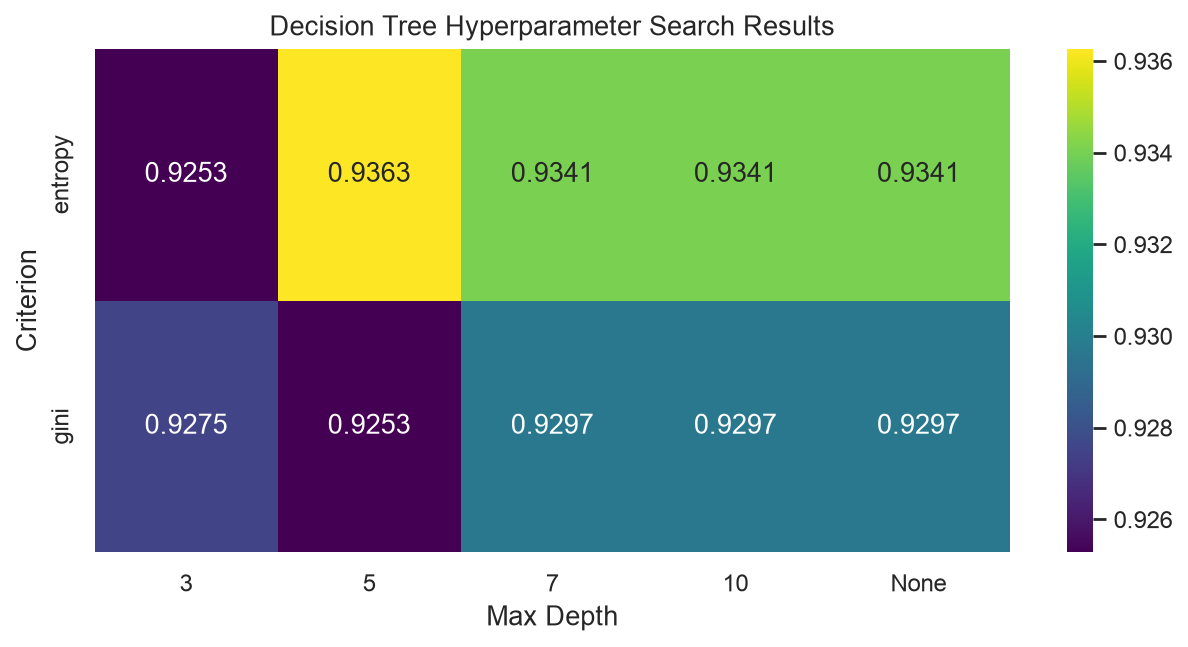
\includegraphics[width=0.65\linewidth]{experiment5_output/eda_reuse/plots/decision_tree_hyperparameter_search_results.png}
\caption{Decision Tree hyperparameter search results across criterion and max depth.}
\end{figure}
Entropy beats Gini at every depth tested, though never by more than half a percentage point, so I would not read too much into the criterion choice on its own. The more interesting pattern is in the depth column: accuracy actually peaks at a shallow \texttt{max\_depth=5} (93.63\%) and then \emph{drops slightly} for depth 7, 10, and unbounded, all of which plateau at exactly 93.41\% -- meaning the extra splits available at depth 7+ are not being used at all beyond what depth 5 already achieves on this 455-row training set. The best configuration selected was criterion=entropy, max\_depth=5, min\_samples\_leaf=2, min\_samples\_split=10, reaching 93.63\% CV accuracy.

% ==========================================================
\section{Random Forest}

\subsection{Baseline Performance}
\begin{table}[h]
\centering
\begin{tabular}{@{}lrrrrr@{}}
\toprule
Model & Accuracy & Precision & Recall & F1 & Train Time (s) \\
\midrule
Random Forest (baseline) & 0.9737 & 1.0000 & 0.9286 & 0.9630 & 0.0503 \\
Random Forest (tuned) & 0.9649 & 1.0000 & 0.9048 & 0.9500 & 0.1045 \\
\bottomrule
\end{tabular}
\caption{Baseline (100 default trees) vs. tuned Random Forest on the test set.}
\end{table}
This is a case where tuning did not help on the held-out test set -- the untuned 100-tree baseline (0.9737 accuracy, 0.9630 F1) actually beats the GridSearchCV-selected configuration (0.9649 accuracy, 0.9500 F1). This is the same phenomenon flagged in Experiment 4 for Logistic Regression: GridSearchCV optimizes cross-validated accuracy on the training folds, not test-set accuracy, so a single 114-row test split can favor a configuration the CV search did not prefer. I trust the CV-based selection (Section 9.2) over this one test-set comparison, since it is averaged over five folds rather than one split of 114 rows.

\subsection{Hyperparameter Tuning}
\begin{lstlisting}
rf_param_grid = {
    "n_estimators": [50, 100, 200],
    "max_depth": [5, 10, None],
    "max_features": ["sqrt", "log2"],
    "bootstrap": [True, False],
}
rf_grid_search = GridSearchCV(
    estimator=RandomForestClassifier(random_state=RANDOM_STATE),
    param_grid=rf_param_grid,
    scoring={"accuracy": "accuracy", "f1": f1_scorer},
    refit="accuracy", cv=cv, n_jobs=-1,
)
\end{lstlisting}

\begin{table}[h]
\centering
\begin{tabular}{@{}rllrr@{}}
\toprule
n\_estimators & Max Depth & Max Features & Avg CV Accuracy (\%) & Avg CV F1 Score \\
\midrule
200 & None & sqrt & 97.14 & 0.9615 \\
200 & 5 & sqrt & 97.14 & 0.9608 \\
50 & 10 & sqrt & 97.14 & 0.9617 \\
200 & 10 & sqrt & 97.14 & 0.9615 \\
50 & 10 & log2 & 96.92 & 0.9584 \\
50 & None & log2 & 96.92 & 0.9584 \\
50 & None & sqrt & 96.92 & 0.9589 \\
100 & 5 & sqrt & 96.92 & 0.9580 \\
\bottomrule
\end{tabular}
\caption{Random Forest hyperparameter evaluation using 5-fold cross-validation (best score per configuration, top 8 of 18 shown).}
\end{table}

\begin{figure}[h]
\centering
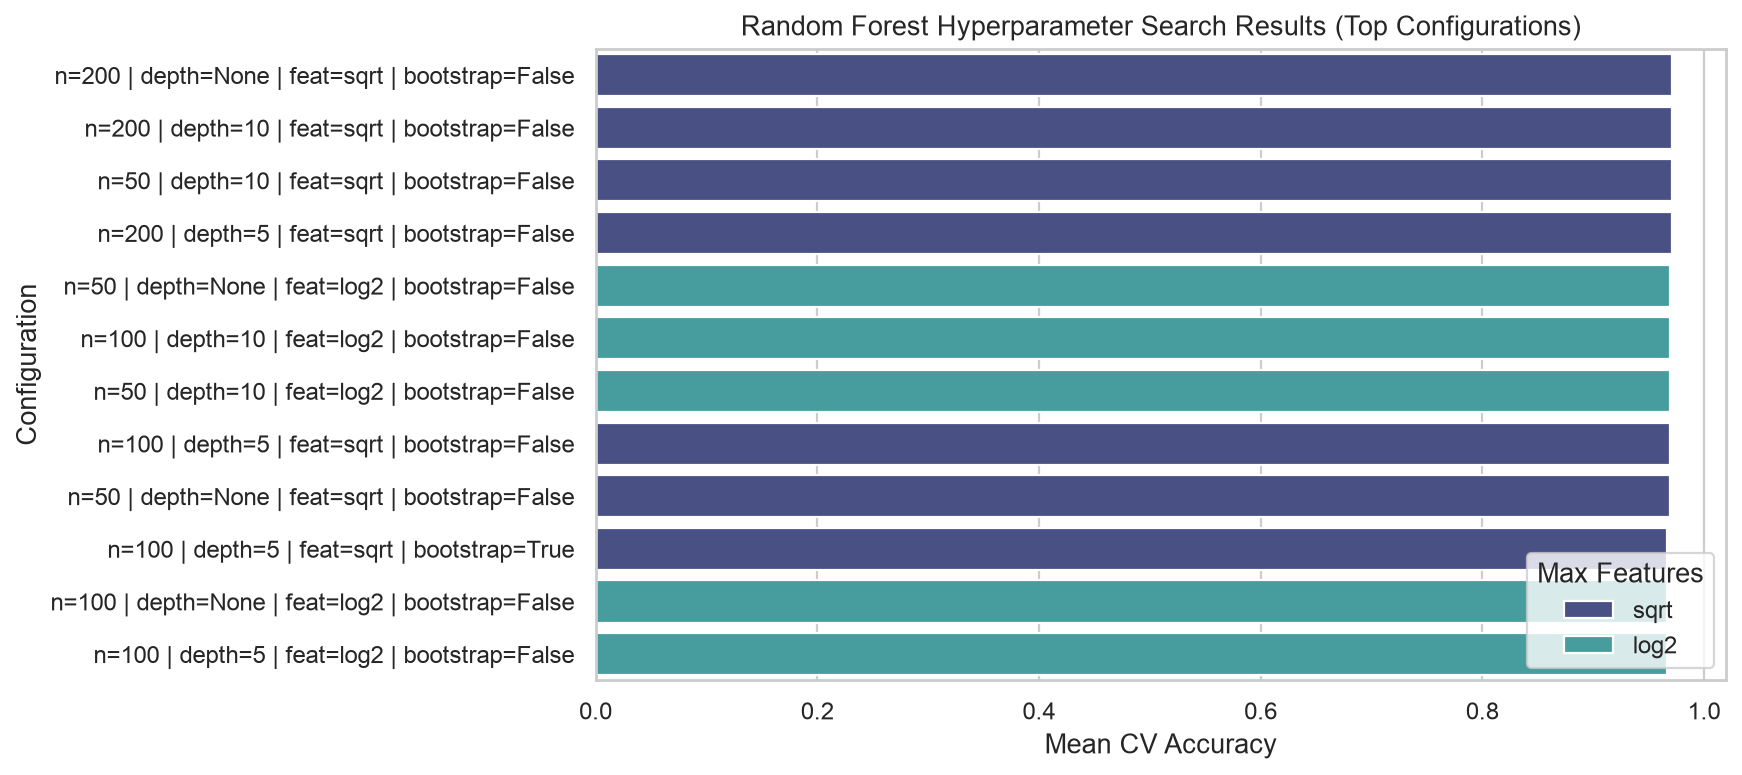
\includegraphics[width=0.75\linewidth]{experiment5_output/eda_reuse/plots/random_forest_hyperparameter_search_results.png}
\caption{Random Forest hyperparameter search results, top 12 configurations by mean CV accuracy.}
\end{figure}
The \texttt{max\_features=sqrt} setting dominates the top of the table -- every one of the four best configurations uses \texttt{sqrt} rather than \texttt{log2}, even though for 30 features the two only differ by a couple of candidate features per split ($\sqrt{30}\approx5$ vs.\ $\log_2 30\approx5$, so this is a closer call than it looks at first glance, but \texttt{sqrt} still wins consistently). The selected configuration was \texttt{n\_estimators=200}, \texttt{max\_depth=5}, \texttt{max\_features=sqrt}, \texttt{bootstrap=False}, reaching 97.14\% CV accuracy -- notably \texttt{bootstrap=False} won out, meaning each tree saw the full training set rather than a bootstrap resample, with the randomness coming entirely from feature subsampling at each split.

% ==========================================================
\section{Hyperparameter Tuning Summary}
\begin{table}[h]
\centering
\small
\begin{tabular}{@{}p{2.1cm}p{2.3cm}p{7cm}p{1.9cm}@{}}
\toprule
Model & Search Method & Best Parameters & Best CV Accuracy \\
\midrule
Decision Tree & GridSearchCV & criterion=entropy, max\_depth=5, min\_samples\_leaf=2, min\_samples\_split=10 & 0.9363 \\
Random Forest & GridSearchCV & n\_estimators=200, max\_depth=5, max\_features=sqrt, bootstrap=False & \textbf{0.9714} \\
\bottomrule
\end{tabular}
\caption{Best hyperparameters found for each model family.}
\end{table}
Both searches converge on the same shallow depth (5), which is a useful cross-check: it is not an artifact of one search space, it is the depth that a 455-row training set with 30 correlated features actually supports before either model starts fitting noise. The Random Forest's best CV accuracy (97.14\%) comfortably beats the Decision Tree's (93.63\%) by 3.51 percentage points, which is the strongest single piece of evidence in this experiment that ensembling is doing real work here, even though it did not show up as a win on the small test-set comparison in Section 9.1.

% ==========================================================
\section{Hyperparameter Selection}
\begin{table}[h]
\centering
\begin{tabular}{@{}p{4.3cm}p{8.5cm}@{}}
\toprule
Parameter & Value \\
\midrule
Decision Tree search space & criterion $\in \{$gini, entropy$\}$; max\_depth $\in \{3,5,7,10,\text{None}\}$; min\_samples\_split $\in \{2,5,10\}$; min\_samples\_leaf $\in \{1,2,4\}$ \\
Selected Decision Tree configuration & criterion=entropy, max\_depth=5, min\_samples\_leaf=2, min\_samples\_split=10 \\
Random Forest search space & n\_estimators $\in \{50,100,200\}$; max\_depth $\in \{5,10,\text{None}\}$; max\_features $\in \{$sqrt, log2$\}$; bootstrap $\in \{$True, False$\}$ \\
Selected Random Forest configuration & n\_estimators=200, max\_depth=5, max\_features=sqrt, bootstrap=False \\
Cross-validation scheme & 5-fold \texttt{StratifiedKFold}, \texttt{random\_state}=42 \\
\bottomrule
\end{tabular}
\caption{Final hyperparameter choices carried into the results below.}
\end{table}

% ==========================================================
\section{Cross-Validation Results}
\begin{table}[h]
\centering
\begin{tabular}{@{}lrrrrrr@{}}
\toprule
Model & Fold 1 & Fold 2 & Fold 3 & Fold 4 & Fold 5 & Average \\
\midrule
Decision Tree & 0.9011 & 0.9560 & 0.9121 & 0.9560 & 0.9560 & 0.9363 \\
Random Forest & 0.9560 & 1.0000 & 0.9451 & 0.9670 & 0.9890 & \textbf{0.9714} \\
\bottomrule
\end{tabular}
\caption{5-fold cross-validation accuracy, tuned models.}
\end{table}

\begin{figure}[h]
\centering
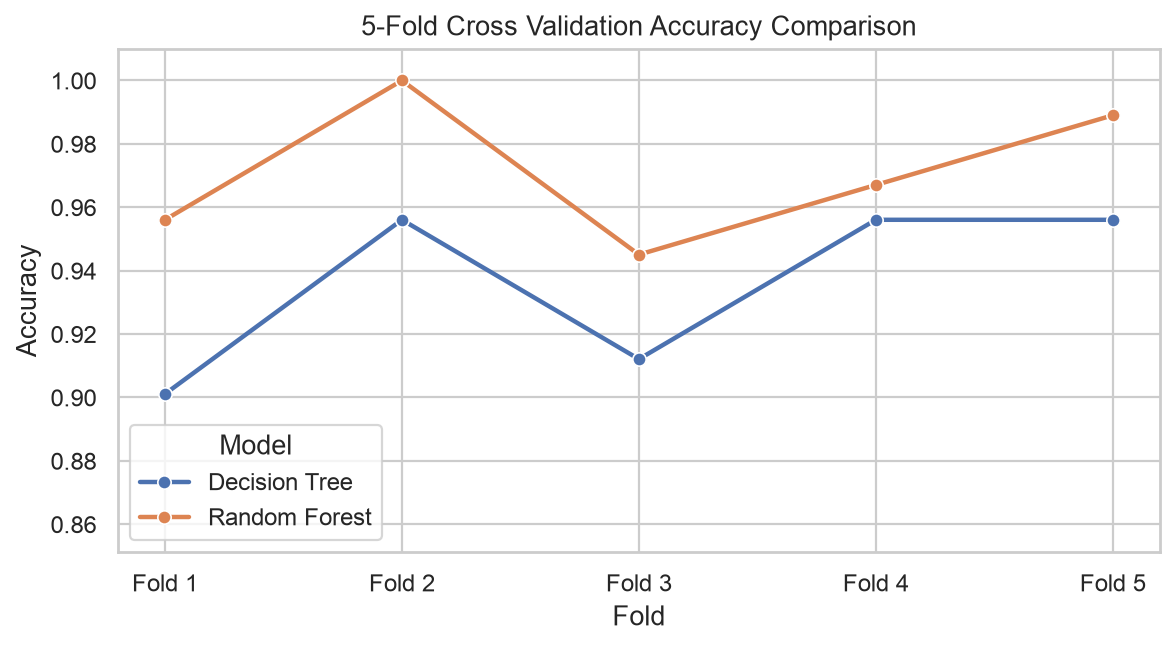
\includegraphics[width=0.6\linewidth]{experiment5_output/eda_reuse/plots/cross_validation_accuracy_comparison.png}
\caption{Per-fold cross-validation accuracy for both tuned models.}
\end{figure}
Random Forest wins every single fold, including a perfect 1.0000 on fold 2, and its worst fold (0.9451) still beats the Decision Tree's best fold (0.9560) in three out of five folds. The Decision Tree's fold 1 score (0.9011) is its weakest by a wide margin, dragging its standard deviation across folds to 0.0245 against the Random Forest's 0.0204 -- so the ensemble is not just more accurate on average here, it is also more consistent fold to fold, which is exactly the variance-reduction behaviour bagging is supposed to deliver.

% ==========================================================
\section{Final Comparison}
\begin{table}[h]
\centering
\small
\begin{tabular}{@{}lrrrrrr@{}}
\toprule
Model & Accuracy & Precision & Recall & F1 & ROC-AUC & Pred.\ Time (s) \\
\midrule
Decision Tree (tuned) & 0.9649 & 1.0000 & 0.9048 & 0.9500 & 0.9744 & \textbf{0.0003} \\
Random Forest (tuned) & 0.9649 & 1.0000 & 0.9048 & 0.9500 & \textbf{0.9937} & 0.0041 \\
\bottomrule
\end{tabular}
\caption{Final held-out test-set comparison.}
\end{table}

\begin{figure}[h]
\centering
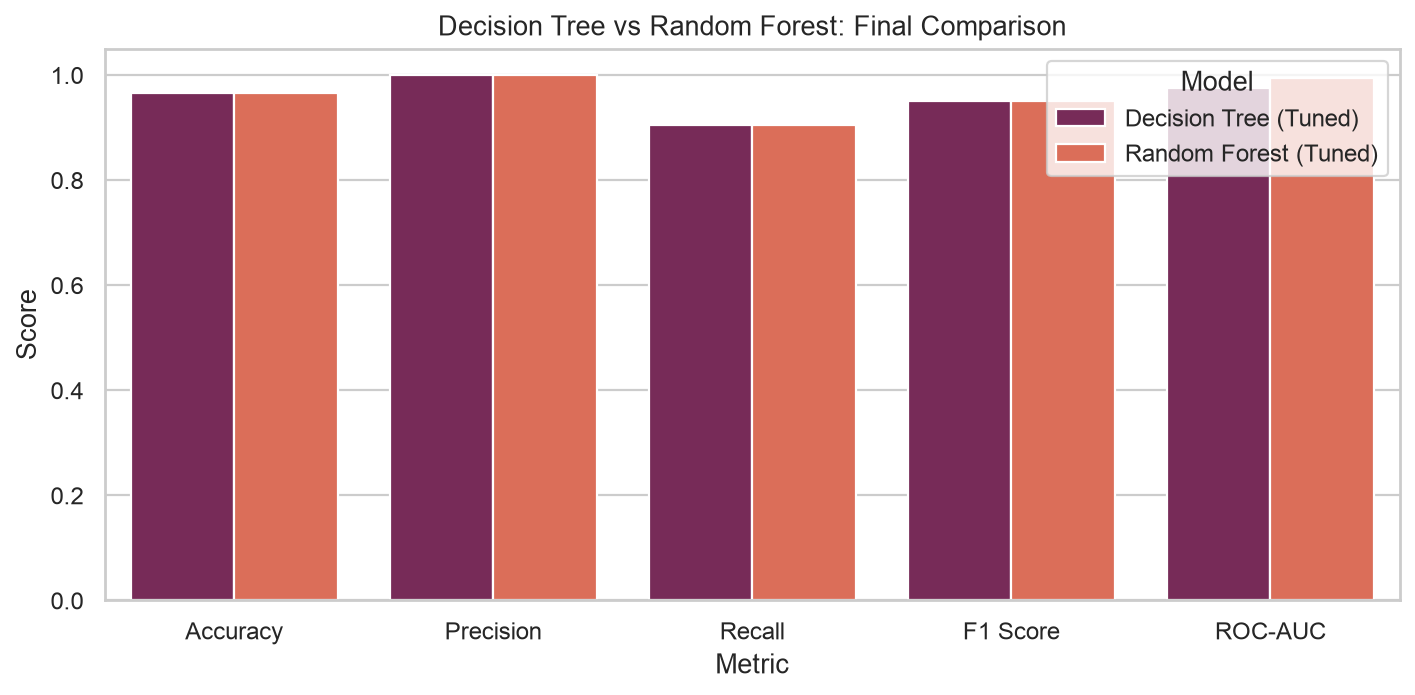
\includegraphics[width=0.7\linewidth]{experiment5_output/eda_reuse/plots/decision_tree_vs_random_forest_comparison.png}
\caption{Final model comparison across metrics.}
\end{figure}
The two tuned models tie exactly on accuracy, precision, recall, and F1 on this particular 114-row test split -- both make the same 4 errors, all false negatives (a malignant case predicted benign), which is the confusion-matrix pattern to watch most closely given the clinical cost of a missed malignancy. Where they separate is ROC-AUC: Random Forest reaches 0.9937 against the Decision Tree's 0.9744, meaning the forest's underlying probability estimates (averaged across 200 trees) rank the two classes more reliably even when the hard 0.5-threshold predictions happen to match.

\begin{figure}[h]
\centering
\begin{subfigure}{0.48\textwidth}
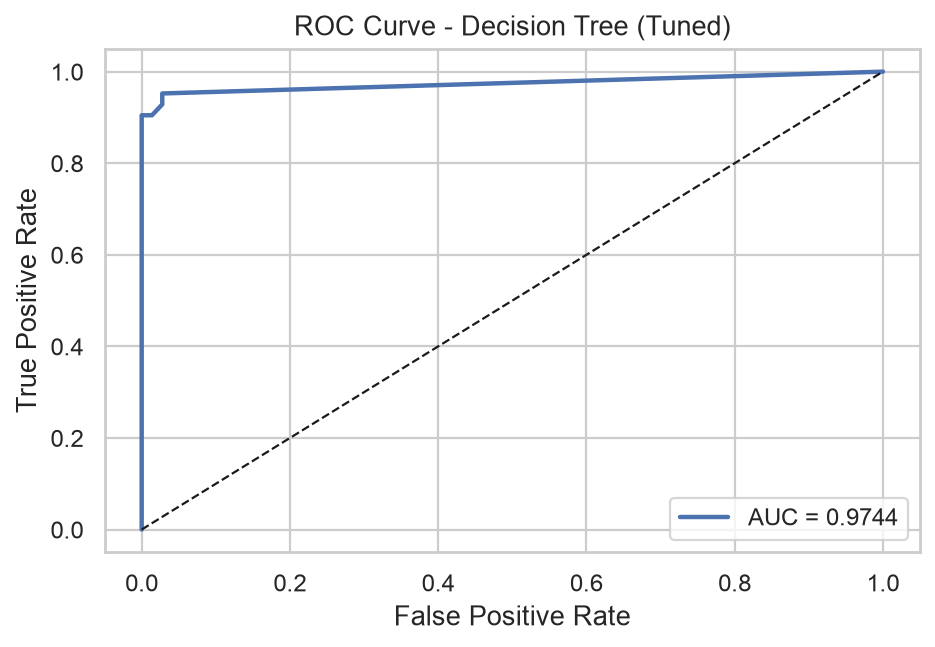
\includegraphics[width=\linewidth]{experiment5_output/eda_reuse/plots/roc_curve_decision_tree_tuned.png}
\caption{ROC, Decision Tree (tuned)}
\end{subfigure}
\hfill
\begin{subfigure}{0.48\textwidth}
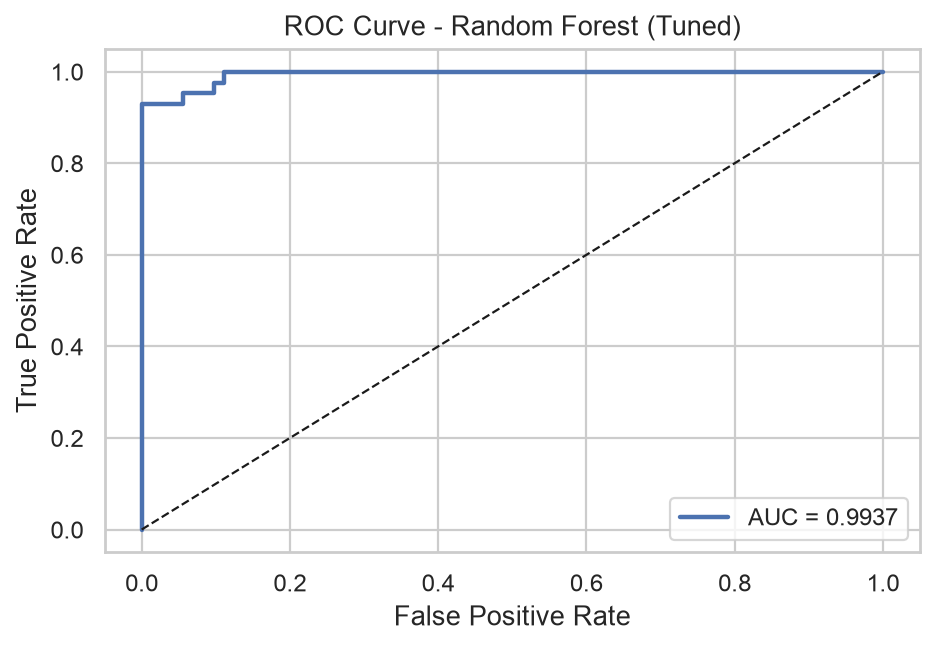
\includegraphics[width=\linewidth]{experiment5_output/eda_reuse/plots/roc_curve_random_forest_tuned.png}
\caption{ROC, Random Forest (tuned)}
\end{subfigure}
\caption{ROC curves for both tuned final models.}
\end{figure}
\begin{figure}[h]
\centering
\begin{subfigure}{0.48\textwidth}
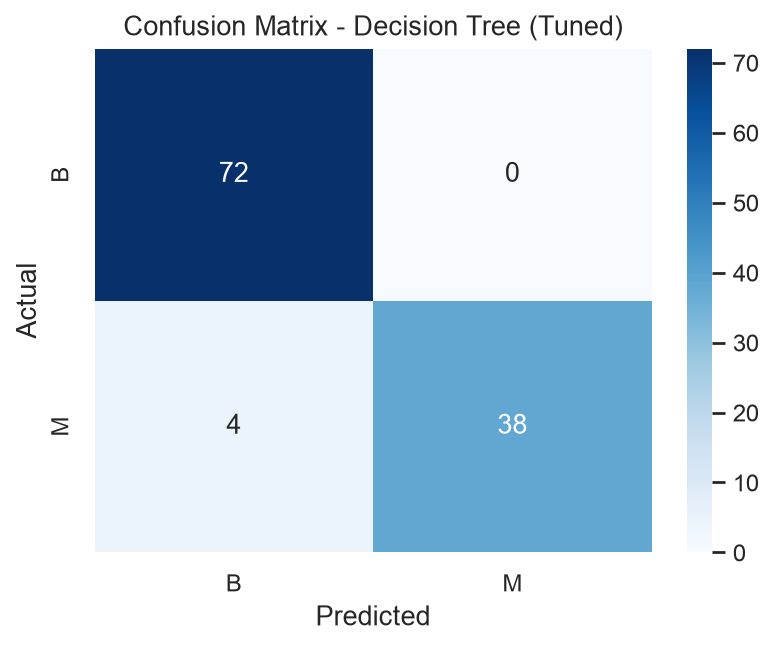
\includegraphics[width=\linewidth]{experiment5_output/eda_reuse/plots/confusion_matrix_decision_tree_tuned.png}
\caption{Confusion matrix, Decision Tree (tuned)}
\end{subfigure}
\hfill
\begin{subfigure}{0.48\textwidth}
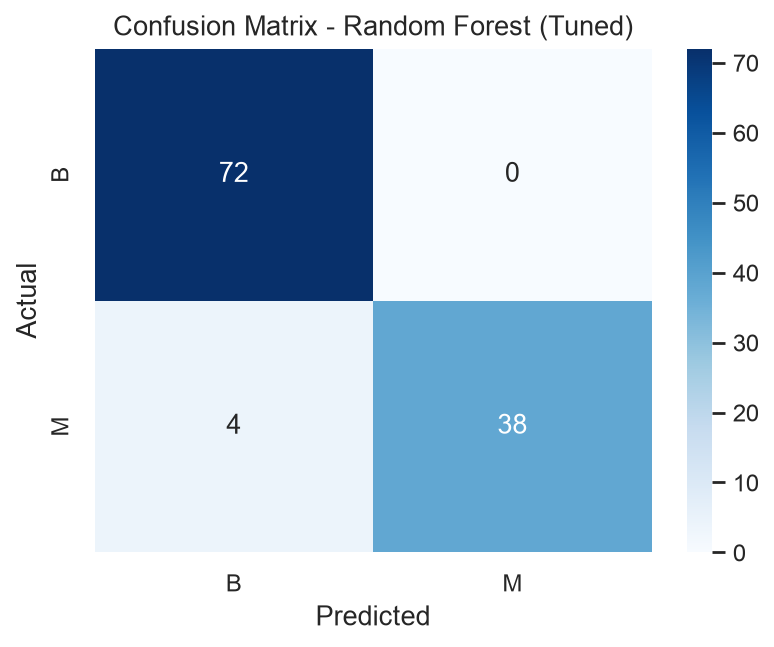
\includegraphics[width=\linewidth]{experiment5_output/eda_reuse/plots/confusion_matrix_random_forest_tuned.png}
\caption{Confusion matrix, Random Forest (tuned)}
\end{subfigure}
\caption{Confusion matrices for both tuned final models.}
\end{figure}
\begin{figure}[h]
\centering
\begin{subfigure}{0.48\textwidth}
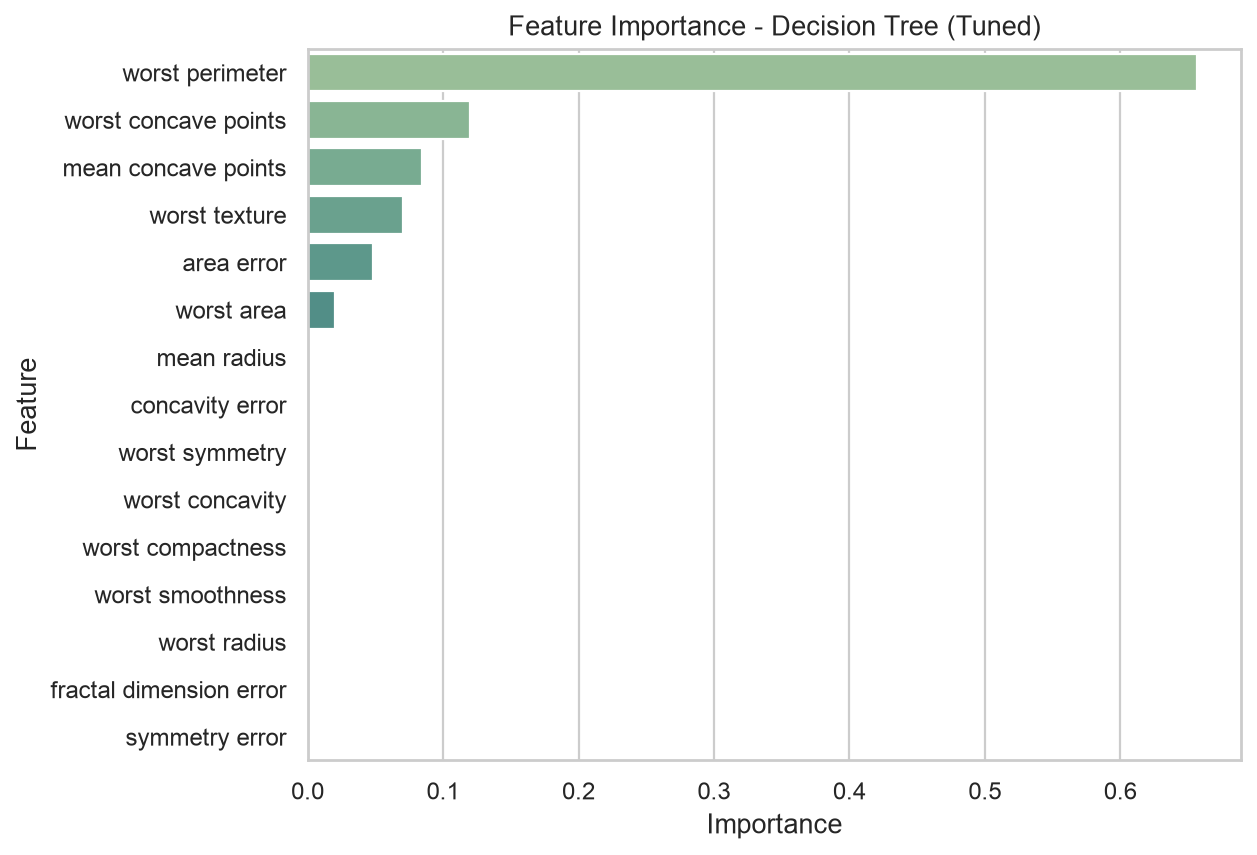
\includegraphics[width=\linewidth]{experiment5_output/eda_reuse/plots/feature_importance_decision_tree_tuned.png}
\caption{Feature importance, Decision Tree (tuned)}
\end{subfigure}
\hfill
\begin{subfigure}{0.48\textwidth}
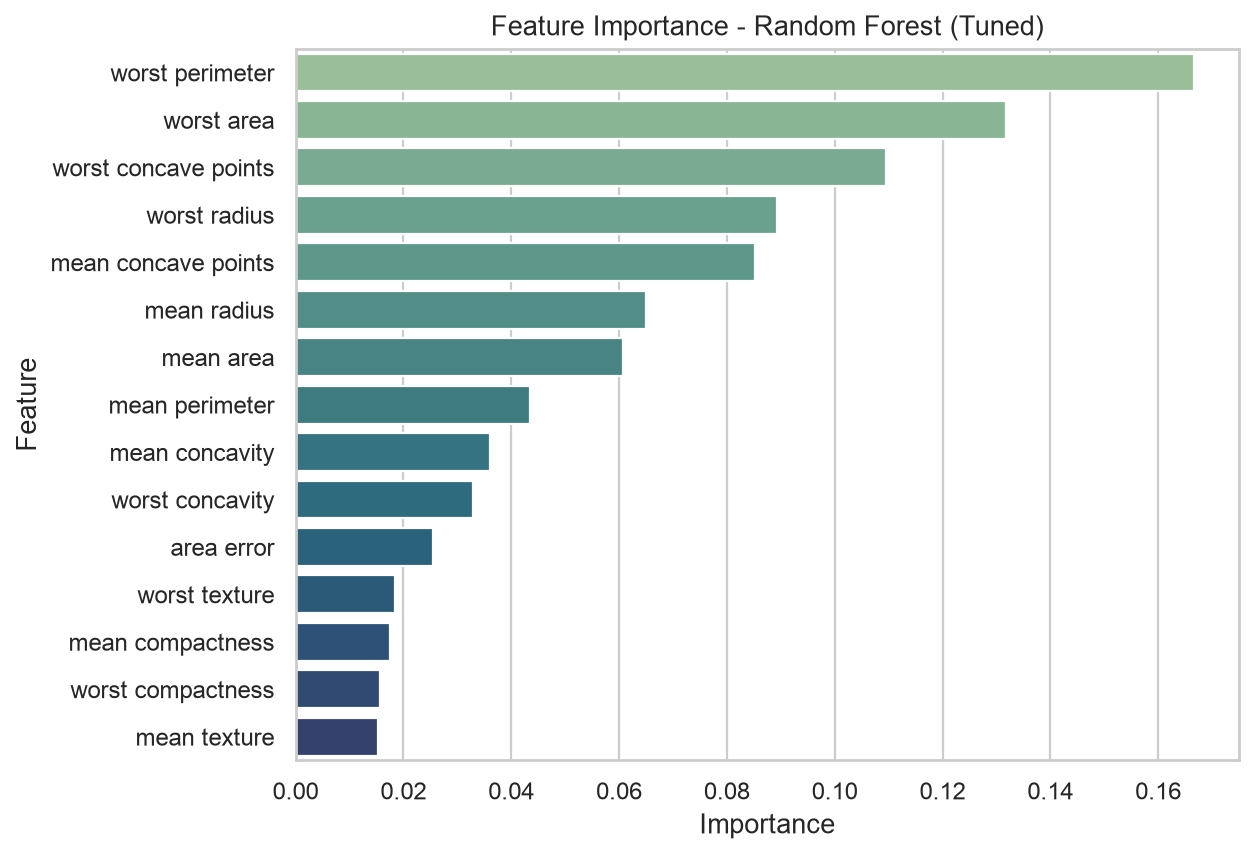
\includegraphics[width=\linewidth]{experiment5_output/eda_reuse/plots/feature_importance_random_forest_tuned.png}
\caption{Feature importance, Random Forest (tuned)}
\end{subfigure}
\caption{Feature importance rankings for both tuned final models.}
\end{figure}
The feature-importance plots are, to me, the clearest illustration of what the ensemble is actually doing differently. The tuned Decision Tree puts roughly 65\% of its total importance on a single feature, \texttt{worst perimeter}, with \texttt{worst concave points} and \texttt{mean concave points} a distant second and third and most of the remaining 30 features contributing exactly zero -- the tree found one dominant split and mostly rode it. The Random Forest's importances are far more distributed: \texttt{worst perimeter} still leads, but at roughly 0.17 rather than 0.65, followed closely by \texttt{worst area} (0.13), \texttt{worst concave points} (0.11), \texttt{worst radius} (0.09), and \texttt{mean concave points} (0.085), with a long tail of a dozen more features still making a visible contribution. Restricting each split to a random feature subset forces different trees to rely on different, correlated stand-ins for ``tumor size'' (radius, perimeter, area all measure roughly the same thing), which is exactly why the importance spreads out instead of concentrating on whichever single feature happened to win the very first split.
\begin{figure}[h]
\centering

\includegraphics[width=0.6\linewidth]{experiment5_output/eda_reuse/plots/time_comparison.png}
\caption{Training and prediction time comparison.}
\end{figure}
The timing gap is the clearest practical trade-off in this experiment: the tuned Random Forest takes roughly 41$\times$ longer to predict than the tuned Decision Tree (0.0041s vs.\ 0.0003s) because a prediction requires evaluating all 200 trees and combining their votes, against one root-to-leaf walk for the single tree. On a 114-row test set neither number is remotely a bottleneck, but the gap would matter at production scale.

% ==========================================================
\section{Comparative Analysis}
\begin{table}[h]
\centering
\begin{tabular}{@{}lll@{}}
\toprule
Criterion & Decision Tree & Random Forest \\
\midrule
Accuracy (test set) & Tied & Tied \\
Accuracy (5-fold CV average) & Lower (0.9363) & Higher (0.9714) \\
Model Complexity & Low (single tree, depth 5) & High (200 trees, depth 5 each) \\
Training Time & Very low (0.0026s tuned) & Moderate (0.1045s tuned) \\
Prediction Time & Very low (0.0003s) & Higher (0.0041s) \\
Interpretability & High (single rule path) & Low (averaged over 200 trees) \\
\bottomrule
\end{tabular}
\caption{Qualitative model comparison.}
\end{table}

\subsection{Observations}
\begin{itemize}[nosep]
  \item \textbf{Best-performing classifier:} on the held-out test set the two tuned models are indistinguishable on accuracy, precision, recall, and F1; Random Forest only pulls ahead on ROC-AUC (0.9937 vs.\ 0.9744) and on the 5-fold CV average (0.9714 vs.\ 0.9363). Given that the CV average is estimated over five folds rather than one 114-row split, I would call Random Forest the more trustworthy choice even though the test-set metrics alone would suggest a tie.
  \item \textbf{Effect of hyperparameter tuning:} tuning helped the Decision Tree unambiguously (accuracy 0.9298 $\to$ 0.9649) but did not help the Random Forest on this particular test split (0.9737 $\to$ 0.9649, a drop) -- both outcomes are consistent with GridSearchCV optimizing CV accuracy, not test accuracy, and the effect is simply more visible for the Random Forest because its untuned baseline (100 default trees) happened to already be strong.
  \item \textbf{Depth sensitivity:} both searches independently converged on \texttt{max\_depth=5} as optimal, and the Decision Tree's own CV accuracy actually plateaus (and does not further improve) past depth 7 -- the practical implication is that this dataset's true decision boundary does not require much tree depth to capture, and pushing depth further only adds capacity to memorize noise.
  \item \textbf{Bias--variance trade-off:} the tuned Decision Tree's CV train--test accuracy gap is 0.0467, while the tuned Random Forest's is 0.0286 -- about 39\% smaller. That gap reduction, together with the Random Forest's lower per-fold standard deviation (0.0204 vs.\ 0.0245), is the most direct quantitative evidence in this experiment that bagging plus feature-subsampling is reducing variance the way the theory predicts.
\end{itemize}

% ==========================================================
\section{Observation Questions}

\textbf{How does tree depth affect overfitting in Decision Trees?}\\
The depth sweep run for this experiment (max\_depth $\in \{1,2,\dots,20,\text{None}\}$, Figure~\ref{fig:overfitting-curve}) shows training accuracy climbing steadily to a perfect 1.0000 as depth grows unconstrained, while test accuracy peaks at 0.9386 around max\_depth=7 and then \emph{declines slightly} and flattens at 0.9298 for every depth from 8 up to unbounded. At max\_depth=1 the tree scores 0.9297 train / 0.8772 test (both low, since a one-split ``stump'' cannot capture much structure); at max\_depth=None it scores 1.0000 train / 0.9298 test, a 7.02-point train--test gap. The pattern is textbook: once the tree has enough depth to separate the training folds perfectly, every additional split only helps memorize training-set idiosyncrasies rather than generalize further.

\begin{figure}[h]
\centering
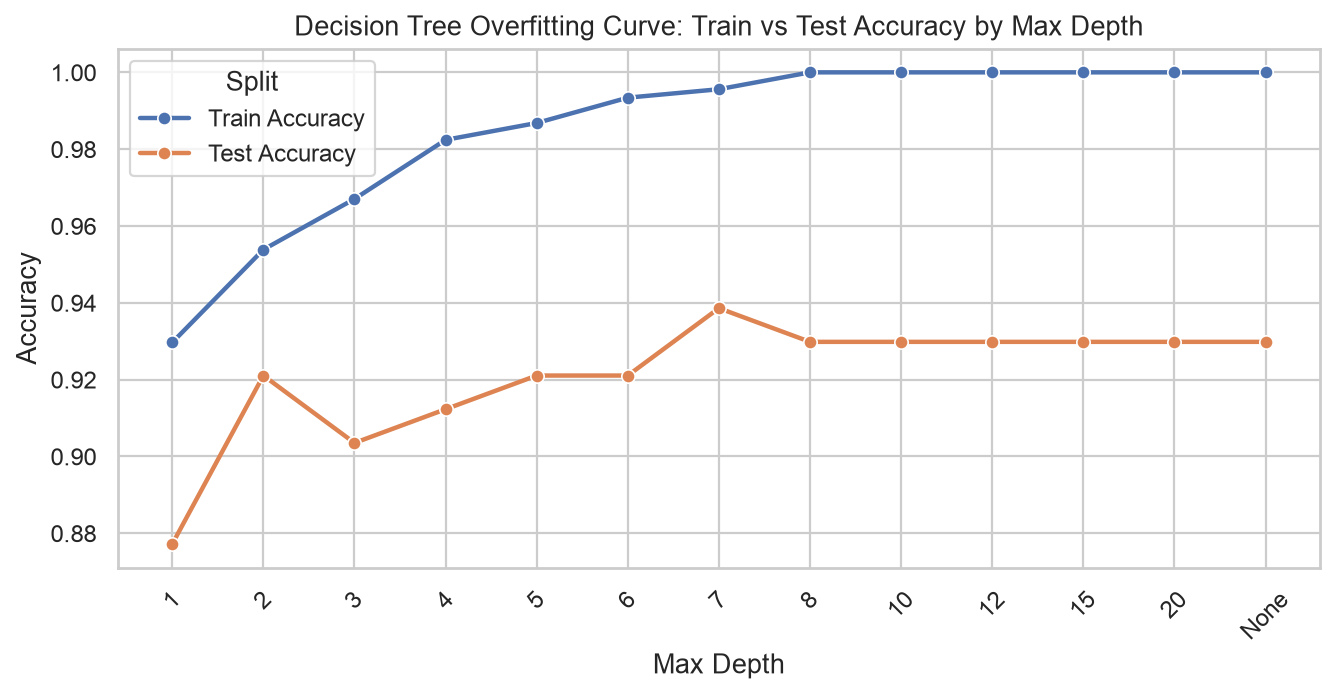
\includegraphics[width=0.75\linewidth]{experiment5_output/eda_reuse/plots/decision_tree_overfitting_curve.png}
\caption{Decision Tree train vs.\ test accuracy across max\_depth values.}
\label{fig:overfitting-curve}
\end{figure}

\textbf{Which hyperparameter had the greatest impact on performance?}\\
Measuring the spread in best CV accuracy as each hyperparameter is varied (holding the others at their best-found value): for the Decision Tree, \texttt{max\_depth} produced a swing of 0.88 percentage points, more than \texttt{criterion}, \texttt{min\_samples\_split}, or \texttt{min\_samples\_leaf} individually. For the Random Forest, \texttt{bootstrap} produced the widest swing at 0.44 percentage points, ahead of \texttt{n\_estimators}, \texttt{max\_depth}, and \texttt{max\_features}. Neither swing is large in absolute terms -- both search spaces were already fairly well-behaved -- but \texttt{max\_depth} clearly matters more for the single tree (it is the only thing standing between the tree and the overfitting shown in Figure~\ref{fig:overfitting-curve}), while for the forest, whether each tree sees a bootstrap resample or the full training set mattered slightly more than how many trees or how deep they were allowed to go.

\textbf{How does Random Forest improve generalization?}\\
Three independent numbers in this experiment all point the same direction. The CV train--test accuracy gap is narrower for the Random Forest (0.0286) than for the Decision Tree (0.0467). The 5-fold CV accuracy average is higher for the forest (0.9714 vs.\ 0.9363). And the per-fold standard deviation is lower for the forest (0.0204 vs.\ 0.0245), meaning its performance is not just better on average but more consistent fold to fold. All three are consistent with the theoretical mechanism: averaging predictions across many trees that are decorrelated by bootstrap resampling and random feature subsampling cancels out the idiosyncratic errors any single tree makes, without materially increasing bias, since each individual tree in the forest is itself no more constrained (same max\_depth=5) than the standalone tuned tree.

\textbf{Did ensemble learning always improve performance? Why or why not?}\\
No -- and this experiment produced a concrete counterexample. On the held-out test set, the tuned Decision Tree and tuned Random Forest are exactly tied on F1 (0.9500 vs.\ 0.9500) and every other threshold-based metric, and the untuned Random Forest baseline actually scored \emph{higher} on the test set (0.9737 accuracy) than the tuned Random Forest (0.9649). Ensembling is not guaranteed to help whenever a single well-regularized tree already captures the decision boundary well -- which is exactly what happened here once both models were constrained to max\_depth=5 -- or when the specific test split happens to favor a configuration the CV search did not select. The place ensembling clearly did help was generalization stability (the CV average and per-fold variance discussed above), not the raw test-set score on this one 114-row split.

% ==========================================================
\section{Discussion}
The most useful result in this experiment is not which model ``won'' -- on the test set they tied -- but the fact that the two evaluation methods (test-set comparison and 5-fold CV) disagree, and that disagreement is itself informative. The test set is a single 114-row sample; the CV average is effectively five independent 91-row test sets, averaged. When the two disagree, as they do here (test set: tied; CV: Random Forest ahead by 3.5 points), I trust the CV number more, because it is far less sensitive to which particular rows happened to land in the test split. This mirrors exactly the same tension found in Experiment 4 between Logistic Regression and SVM, and I think it is a pattern worth expecting on any dataset small enough that a single test split carries meaningful sampling variance -- 114 test rows is not a lot of rows to draw a confident conclusion from.

The main limitation of this experiment is dataset size: 569 total samples is enough to get a clean signal from 5-fold cross-validation, but it is small enough that a single test-set comparison (Section 10) is genuinely noisy, as the disagreement with the CV results demonstrates. A second limitation is that the hyperparameter search spaces, while reasonably wide, were not exhaustive -- neither grid explored the interaction between \texttt{max\_depth} and \texttt{min\_samples\_leaf} at every combination for the forest the way it did for the tree, since the forest's grid held \texttt{min\_samples\_leaf} fixed at its default to keep the search tractable at 5-fold CV.

If extending this experiment, I would add a learning-curve analysis (accuracy vs.\ training-set size) alongside the depth sweep already produced, since that would help separate ``this dataset is too small to fully exploit the Random Forest's advantage'' from ``the advantage genuinely caps out around 97\% CV accuracy regardless of data size'' -- the current results are consistent with either explanation.

% ==========================================================
\section{Conclusion}
Both models reach the same test-set performance after tuning (96.49\% accuracy, 0.9500 F1), which on its own would suggest the ensemble adds nothing here. But the 5-fold cross-validation results tell a more complete story: Random Forest's CV accuracy (97.14\%) beats the Decision Tree's (93.63\%) by 3.51 points, its train--test gap is 39\% narrower (0.0286 vs.\ 0.0467), and its ROC-AUC on the test set is meaningfully higher (0.9937 vs.\ 0.9744) even where the hard classification decisions tie. I read this as ensembling doing exactly what the theory predicts -- reducing variance and improving the reliability of the underlying probability estimates -- without necessarily moving the single-split test-set accuracy, which is too coarse a measurement to detect a variance reduction this size. If deployment latency and interpretability were the priority, the tuned Decision Tree (0.0003s prediction, one readable rule path, identical test-set metrics) would be the practical choice; if the goal is the most reliable estimate of malignancy probability across unseen patients, the Random Forest's higher and more stable cross-validated accuracy makes it the better bet.

% ==========================================================
\section{References}
\begin{enumerate}[label={[\arabic*]}]
\item F. Pedregosa et al., ``Scikit-learn: Machine Learning in Python,'' \emph{Journal of Machine Learning Research}, vol. 12, pp. 2825--2830, 2011.
\item L. Breiman, ``Random Forests,'' \emph{Machine Learning}, vol. 45, no. 1, pp. 5--32, 2001.
\item W. H. Wolberg, W. N. Street, and O. L. Mangasarian, ``Breast Cancer Wisconsin (Diagnostic) Data Set,'' UCI Machine Learning Repository, 1995. [Online]. Available: \url{https://archive.ics.uci.edu/dataset/17/breast+cancer+wisconsin+diagnostic}
\item A. G\'eron, \emph{Hands-On Machine Learning with Scikit-Learn, Keras, and TensorFlow}, 3rd ed. Sebastopol, CA: O'Reilly Media, 2022.
\item C. M. Bishop, \emph{Pattern Recognition and Machine Learning}. New York: Springer, 2006.
\item Scikit-learn Developers, ``Decision Trees,'' \emph{Scikit-learn Documentation}. [Online]. Available: \url{https://scikit-learn.org/stable/modules/tree.html}
\item Scikit-learn Developers, ``Ensemble Methods,'' \emph{Scikit-learn Documentation}. [Online]. Available: \url{https://scikit-learn.org/stable/modules/ensemble.html}
\end{enumerate}

\end{document}
